% #############################################################################
% This is Chapter 3
% !TEX root = ../main.tex
% #############################################################################
% Change the Name of the Chapter i the following line
\fancychapter{Related Work}
\cleardoublepage
% The following line allows to ref this chapter
\label{chap:architecture}

This chapter reviews existing work in aerial image segmentation datasets, ranging from traditional semantic and instance segmentation datasets to specialized referring segmentation datasets and historical imagery applications.

% #############################################################################
\section{Aerial Image Segmentation Datasets}

The foundation for effective aerial image understanding lies in comprehensive datasets that capture the diversity and complexity of remote sensing imagery. This section examines the evolution from traditional segmentation datasets to specialized referring segmentation datasets and historical imagery applications.

\subsection{Traditional Aerial Segmentation Datasets}

Early efforts in aerial image segmentation focused on providing basic semantic and instance annotations for common remote sensing tasks. These foundational datasets established important benchmarks and annotation standards that continue to influence modern dataset construction.

The iSAID dataset represents a significant advancement in instance segmentation for aerial imagery, providing detailed object-level annotations across diverse geographical regions. Building upon the DOTA dataset foundation, iSAID offers precise instance boundaries for 15 different categories commonly found in aerial imagery, including vehicles, buildings, and infrastructure elements. The dataset contains over 655,000 annotated instances across high-resolution imagery, establishing a comprehensive benchmark for instance-level understanding in remote sensing applications.

\begin{figure}[htbp]
\centering
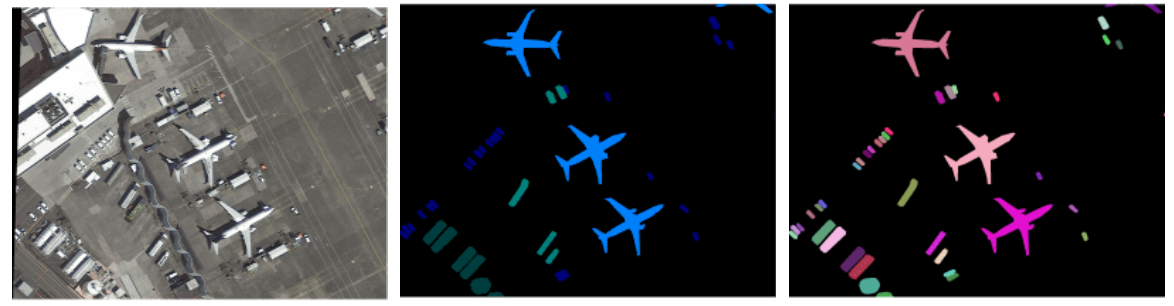
\includegraphics[width=0.8\textwidth]{Images/isaid_examples.png}
\caption{iSAID dataset examples showing instance segmentation annotations for aerial imagery, demonstrating the detailed object-level boundaries across diverse geographical contexts.}
\label{fig:isaid_examples}
\end{figure}

The LoveDA dataset takes a complementary approach, focusing on semantic segmentation for land cover and infrastructure analysis. Unlike instance-based approaches, LoveDA provides dense pixel-level annotations for seven primary land cover categories including buildings, roads, water, barren land, forest, agriculture, and background. The dataset emphasizes multi-domain applicability by incorporating both urban and rural imagery collected from different geographical regions, enabling research into domain adaptation techniques for aerial image analysis.

\begin{figure}[htbp]
\centering
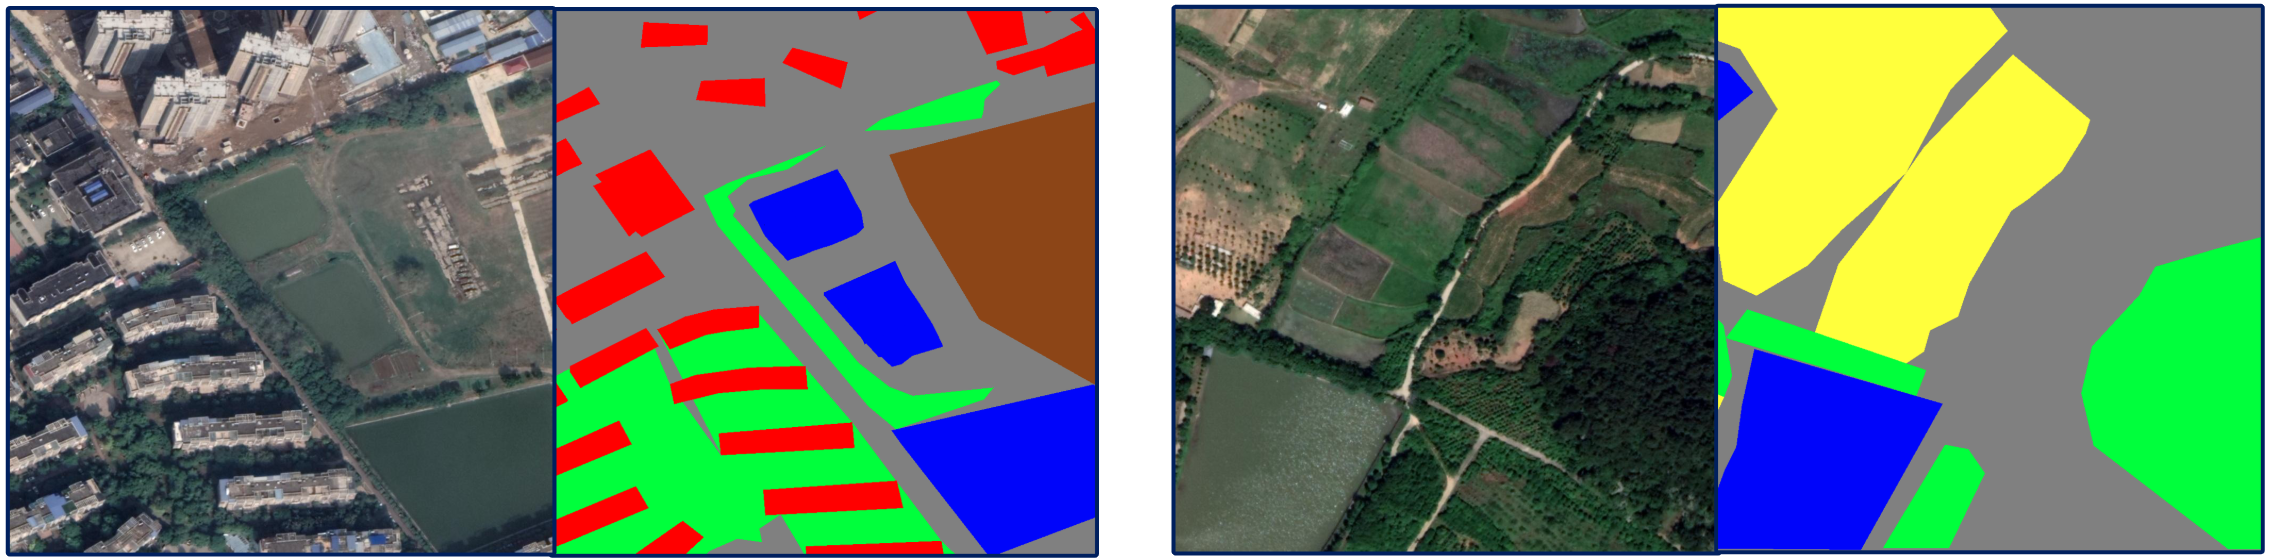
\includegraphics[width=0.8\textwidth]{Images/loveda.png}
\caption{LoveDA dataset examples showing semantic segmentation annotations for land use and land cover classification, highlighting the dense pixel-level labeling approach across urban and rural contexts.}
\label{fig:loveda_examples}
\end{figure}

\subsection{Referring Segmentation Datasets}

Traditional segmentation datasets provide important foundations, but they lack the natural language interface necessary for interactive aerial image analysis. Referring segmentation datasets address this limitation by combining visual annotations with natural language descriptions, enabling text-guided segmentation capabilities.

RefSegRS pioneered the field of referring segmentation for remote sensing imagery, introducing the first dataset to combine aerial imagery with natural language referring expressions. Built upon the SkyScapes dataset foundation, RefSegRS contains 4,420 triplets of images, referring expressions, and corresponding segmentation masks. The dataset focuses on establishing basic referring segmentation capabilities for aerial imagery, with expressions emphasizing spatial relationships, object attributes, and contextual descriptions that are characteristic of remote sensing analysis workflows.

RRSIS-D expanded upon the RefSegRS foundation by introducing larger scale and semi-automated annotation approaches. The dataset contains 17,402 triplets derived from the RSVGD dataset, incorporating Segment Anything Model (SAM) assistance to accelerate annotation generation while maintaining quality standards. RRSIS-D addresses scale limitations of earlier datasets while introducing more diverse expression types across 20 different object categories and seven attribute dimensions, enabling more comprehensive evaluation of referring segmentation approaches.

\begin{figure}[htbp]
\centering
\subfigure[RefSegRS dataset example samples.]{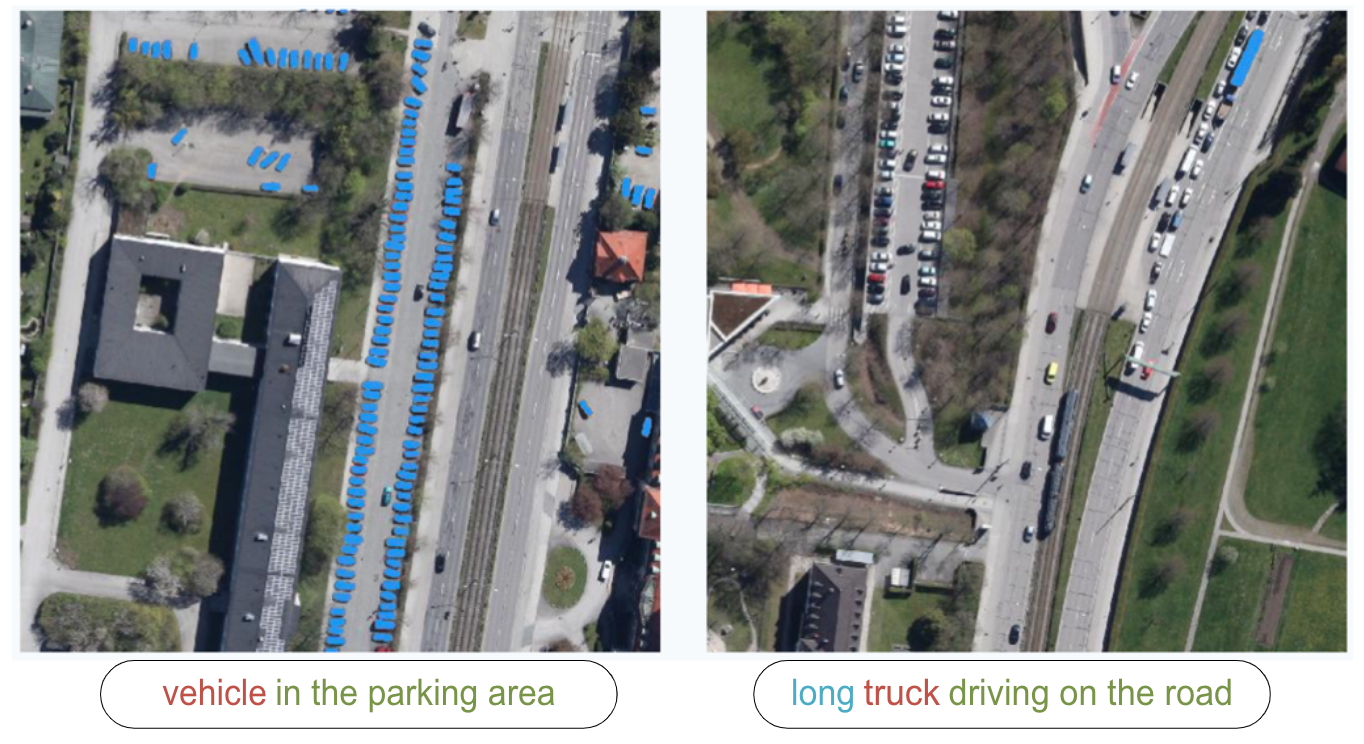
\includegraphics[width=0.45\textwidth]{Images/refsegrs.png}\label{fig:refsegrs}}
\hfill
\subfigure[RRSIS-D dataset example samples.]{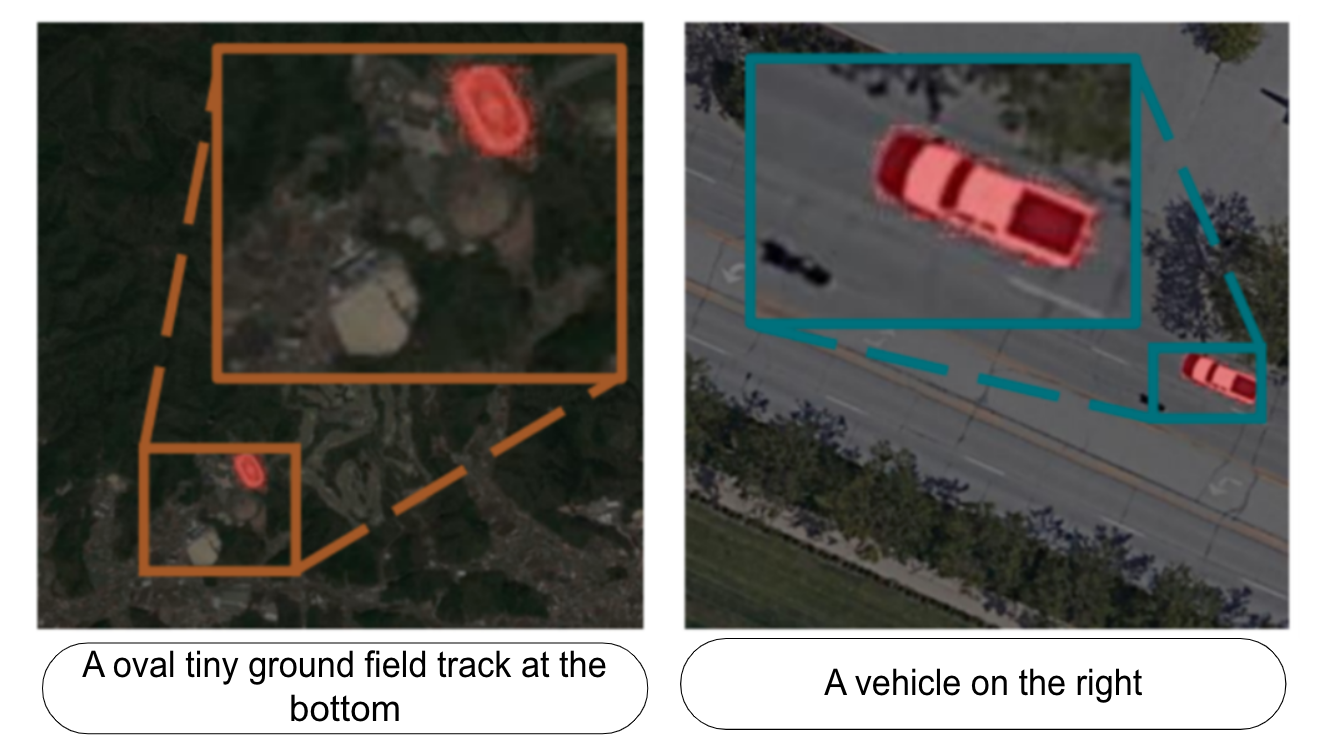
\includegraphics[width=0.45\textwidth]{Images/rrsisd.png}\label{fig:rrsisd}}
\caption{Examples from early aerial referring segmentation datasets showing the evolution from basic referring expressions to more diverse and comprehensive annotation approaches.}
\label{fig:aerial_datasets}
\end{figure}

NWPU-Refer represents the current state-of-the-art in aerial referring segmentation datasets, significantly expanding both scale and annotation sophistication. The dataset contains 49,745 triplets sourced from multiple global aerial imagery collections, providing comprehensive coverage across different geographical regions and imaging conditions. NWPU-Refer introduces enhanced annotation quality through purely manual annotation processes, resulting in more natural and diverse referring expressions. The dataset incorporates 32 object categories with six attribute dimensions, enabling evaluation of fine-grained referring segmentation capabilities that closely match real-world aerial image analysis requirements.

\subsection{Historical Imagery Segmentation}

While contemporary aerial datasets provide important foundations for modern remote sensing analysis, historical imagery represents a largely unexplored domain with significant research and practical value. Historical aerial imagery offers unique insights into temporal changes in land use, urban development patterns, and environmental evolution that cannot be captured through contemporary imagery alone. However, the scarcity of annotated historical datasets has limited progress in this important application area.

The UrbanSatSeg1960 dataset addresses this gap by providing semantic segmentation annotations for historical urban aerial imagery from the 1960s era. This specialized dataset focuses on urban environments captured during a pivotal period of global urbanization, offering ground truth annotations for land cover categories relevant to historical analysis including buildings, roads, vegetation, and open spaces. UrbanSatSeg1960 enables research into historical imagery understanding while providing essential training data for temporal analysis applications that require consistent segmentation capabilities across different imaging eras.

\begin{table}[htbp]
\centering
\caption{Aerial Referring Segmentation (RRSIS) Dataset Comparison}
\label{tab:rrsis_comparison}
\begin{tabular}{@{}llll@{}}
\toprule
\textbf{Feature} & \textbf{RefSegRS} & \textbf{RRSIS-D} & \textbf{NWPU-Refer} \\
\midrule
Size & 4,420 triplets & 17,402 triplets & 49,745 triplets \\
Source & SkyScapes & RSVGD & Multi-source global \\
Annotation & Manual & Semi-auto (SAM) & Manual \\
Resolution & Limited & 800×800 fixed & 1024-2048px \\
Focus & RRSIS & RRSIS & RRSIS \\
Categories & - & 20 & 32 \\
Attributes & 3 & 7 & 6 dimensions \\
\bottomrule
\end{tabular}
\end{table}

\begin{table}[htbp]
\centering
\caption{Source Aerial Dataset Comparison}
\label{tab:source_comparison}
\begin{tabular}{@{}lll@{}}
\toprule
\textbf{Feature} & \textbf{iSAID} & \textbf{LoveDA} \\
\midrule
Size & 655,451 instances & 5,987 images \\
Source & DOTA (re-ann.) & Spaceborne (0.3m) \\
Annotation & Professional & Manual \\
Resolution & High res. & 1024×1024px \\
Focus & Instance Seg. & Land-cover Seg. + UDA \\
Categories & 15 & 7 \\
Attributes & - & Domain labels \\
\bottomrule
\end{tabular}
\end{table}

\begin{table}[htbp]
\centering
\caption{RRSIS Dataset Split Statistics}
\label{tab:rrsis_splits}
\begin{tabular}{@{}llllll@{}}
\toprule
\textbf{Dataset} & \textbf{Total} & \textbf{Training} & \textbf{Validation} & \textbf{Test} & \textbf{Unit} \\
\midrule
RefSegRS & 4,420 & 2,172 (49.1\%) & 431 (9.8\%) & 1,817 (41.1\%) & expressions \\
RRSIS-D & 17,402 & 8,701 (50.0\%) & 3,480 (20.0\%) & 5,221 (30.0\%) & triplets \\
NWPU-Refer & 49,745 & 34,821 (70.0\%) & 4,974 (10.0\%) & 9,950 (20.0\%) & triplets \\
\bottomrule
\end{tabular}
\end{table}

\begin{table}[htbp]
\centering
\caption{Source Dataset Split Statistics}
\label{tab:source_splits}
\begin{tabular}{@{}llllll@{}}
\toprule
\textbf{Dataset} & \textbf{Total} & \textbf{Training} & \textbf{Validation} & \textbf{Test} & \textbf{Unit} \\
\midrule
iSAID & 2,806 & 1,403 (50.0\%) & 468 (16.7\%) & 935 (33.3\%) & images \\
LoveDA & 5,987 & 2,522 (42.1\%) & 1,669 (27.9\%) & 1,796 (30.0\%) & images \\
\bottomrule
\end{tabular}
\end{table}

% #############################################################################
\section{Segmentation Models for Aerial Images}

This section examines the landscape of segmentation models specifically designed for or applicable to aerial imagery analysis, encompassing both semantic segmentation approaches and referring segmentation techniques.

\subsection{Semantic Segmentation Models}

Foundational vision models provide the backbone architectures for aerial image segmentation tasks through powerful feature extraction and mask generation capabilities.

Vision-language models such as CLIP establish crucial connections between visual and textual modalities through contrastive learning, enabling zero-shot classification capabilities that transfer effectively to aerial imagery domains. The learned joint embedding spaces capture semantic relationships that prove valuable for understanding aerial scene content and object categories.

SigLIP represents an advancement in vision-language training methodologies, improving upon CLIP's contrastive approach through more efficient training objectives and enhanced representation learning. These improvements translate to better performance on downstream aerial image understanding tasks where precise visual-textual alignment is critical.

The Segment Anything Model (SAM) provides a foundational approach to semantic segmentation through its prompt-based architecture, as illustrated in Figure~\ref{fig:sam_architecture}. SAM's design incorporates an image encoder that processes input imagery into rich feature representations, a prompt encoder that handles various input modalities including points, boxes, and text, and a mask decoder that generates precise segmentation boundaries. This architecture demonstrates remarkable generalization capabilities across diverse image domains, including aerial imagery, where its ability to process multiple prompt types enables flexible segmentation workflows that can adapt to different user requirements and annotation strategies.

\begin{figure}[htbp]
\centering
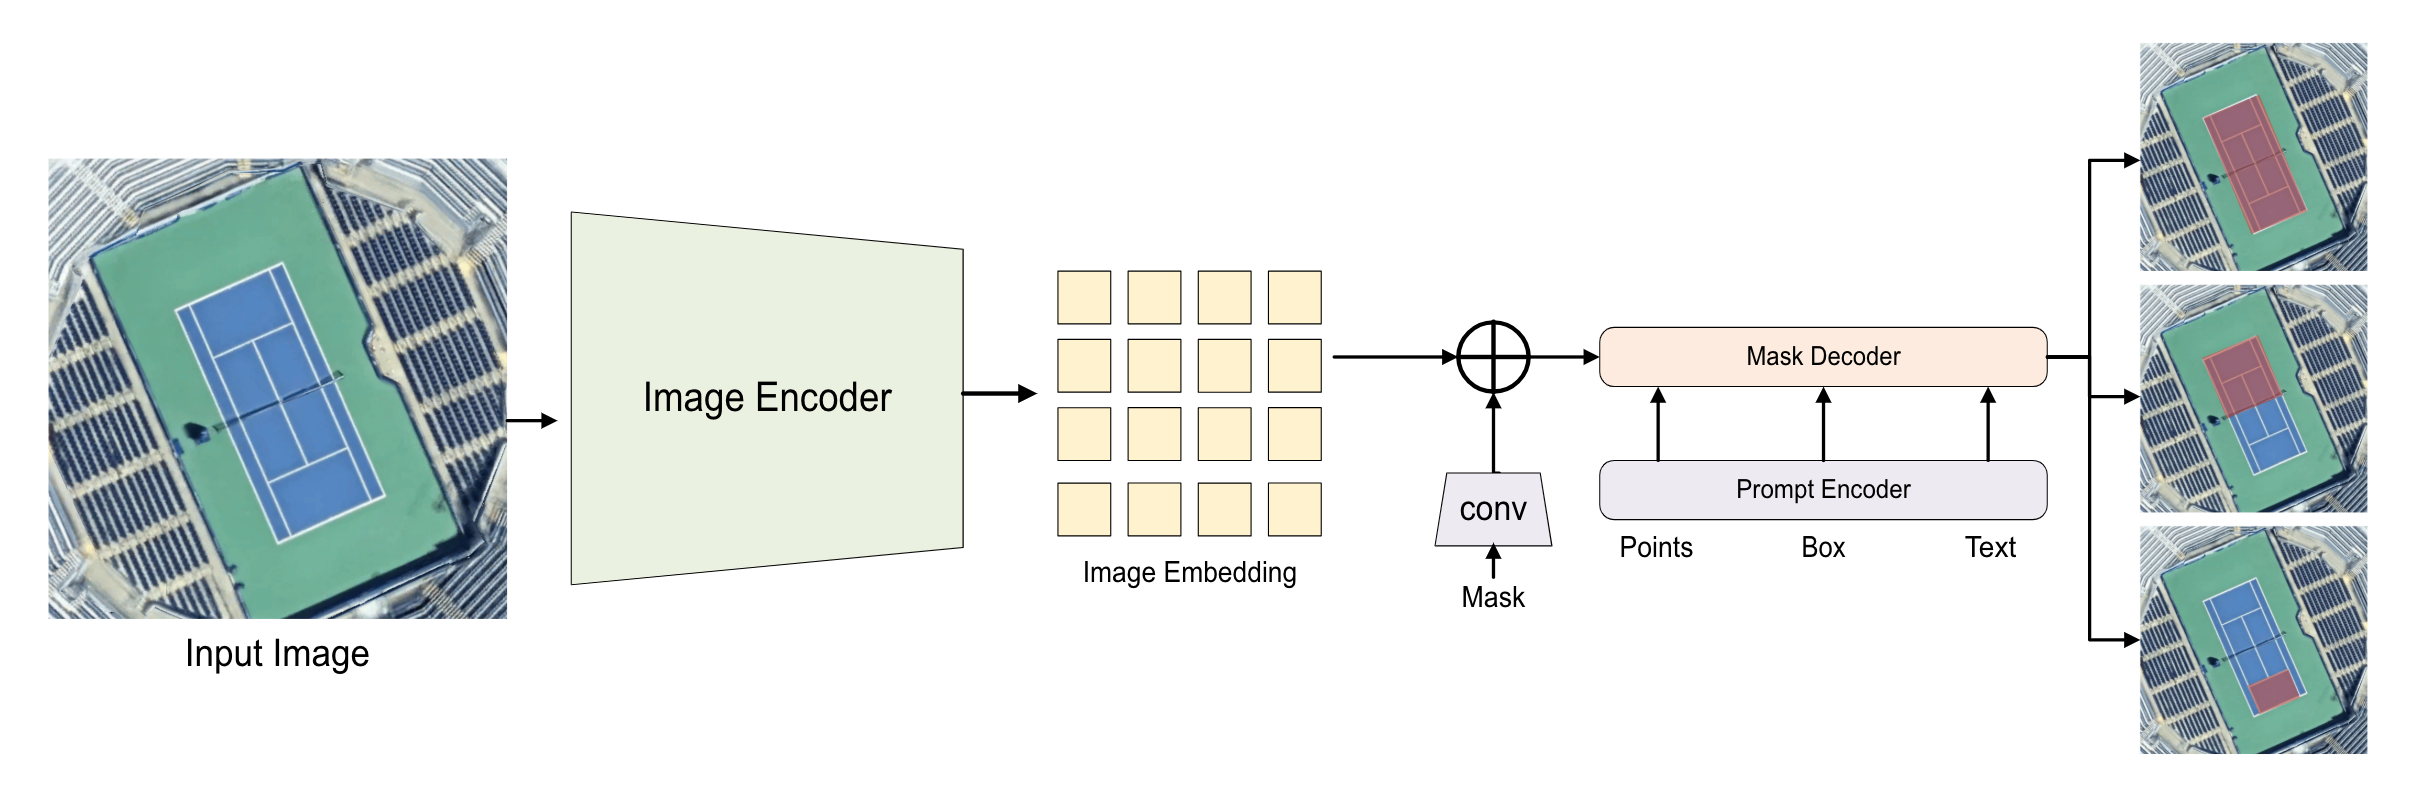
\includegraphics[width=1.0\textwidth]{Images/sam.png}
\caption{Segment Anything Model (SAM) architecture showing the image encoder, prompt encoder, and mask decoder components. The model processes various prompt types including points, boxes, and text to generate precise segmentation masks.}
\label{fig:sam_architecture}
\end{figure}

\subsection{Referring Segmentation Models}

Advanced referring segmentation approaches combine semantic understanding with natural language comprehension to enable text-guided segmentation in aerial imagery contexts.

Previous approaches to language-guided segmentation have established important foundations for referring segmentation in natural images. LAVT introduces attention-based fusion mechanisms that align textual and visual features for precise object localization and segmentation. RMSIN advances multi-scale integration strategies that capture objects at different scales and resolutions. FIANet demonstrates the effectiveness of feature interaction architectures that enable sophisticated text-visual reasoning for segmentation tasks.

RSRefSeg represents a specialized approach designed specifically for aerial referring segmentation, as shown in Figure~\ref{fig:rsrefseg_architecture}. The architecture integrates SigLIP2 vision-language encoders with SAM mask decoders through custom prompter networks that process text-guided segmentation requests. The dual-pathway design processes both local token-level and global sentence-level text-visual interactions, generating sparse and dense prompts that enable precise aerial image segmentation guided by natural language descriptions. This architecture addresses the unique challenges of aerial imagery analysis, including varied object scales, complex spatial relationships, and domain-specific terminology requirements.

\begin{figure}[H]
\centering
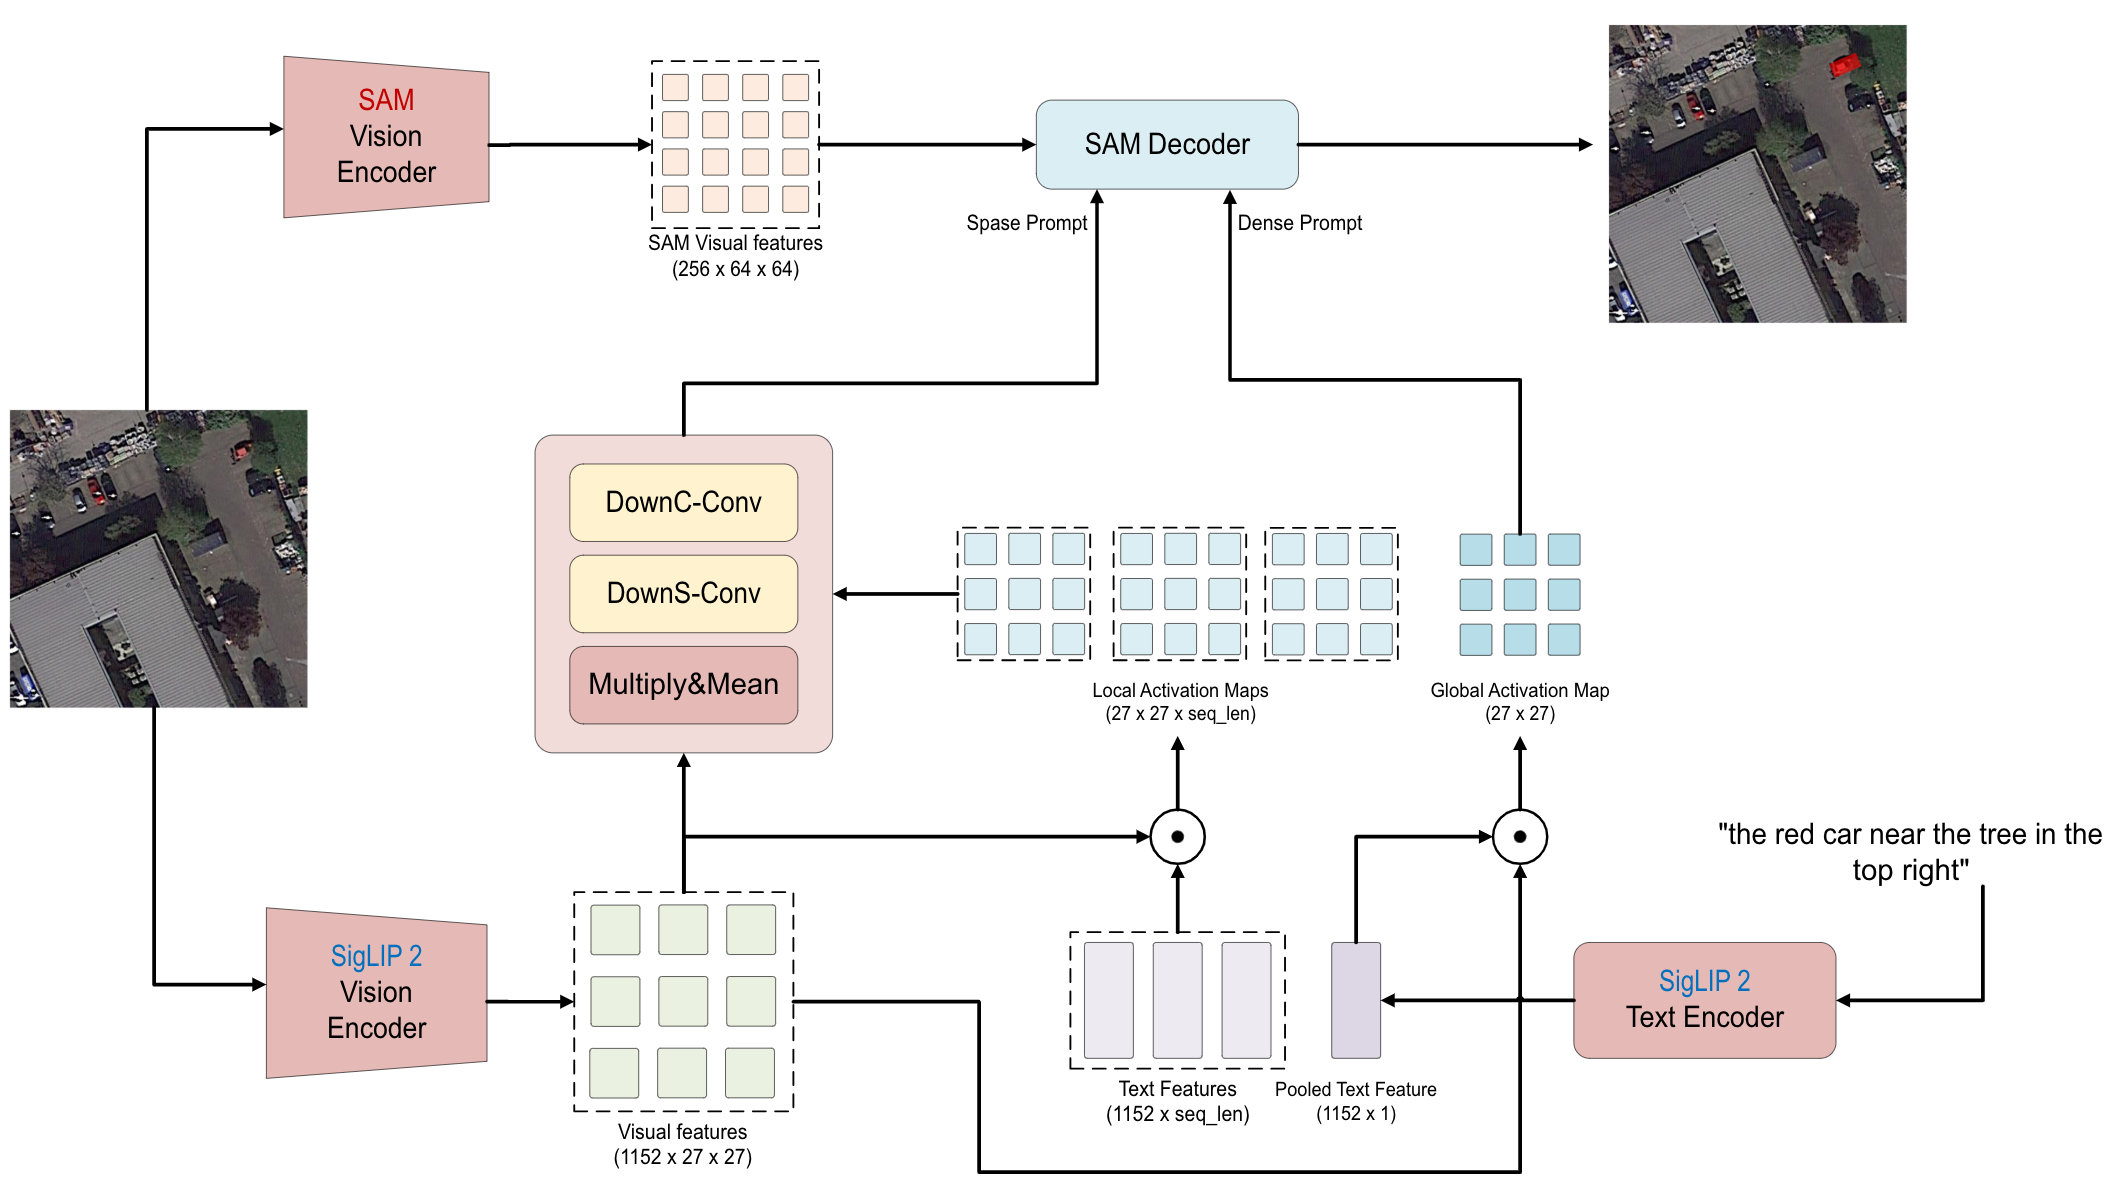
\includegraphics[width=\textwidth]{Images/clipsam.png}
\caption{RSRefSeg architecture overview showing the integration of SigLIP2 vision-language encoder with SAM mask decoder through custom prompter networks for text-guided segmentation. The dual-pathway design processes both local (token-level) and global (sentence-level) text-visual interactions to generate sparse and dense prompts for precise aerial image segmentation.}
\label{fig:rsrefseg_architecture}
\end{figure}

% #############################################################################
\section{Overview}

[Synthesis of all related work - gaps identified and how this work addresses them] % \cite{placeholder_synthesis}